\documentclass[12pt,a4]{article}
\usepackage[utf8]{inputenc}
\usepackage[portuguese,brazilian]{babel}
\usepackage[lmargin=3cm,tmargin=3cm,rmargin=2cm,bmargin=2cm]{geometry}
\usepackage[T1]{fontenc}
\usepackage{amsmath,amsthm,amsfonts,amssymb,dsfont,mathtools,blindtext}
\usepackage{graphicx}
\usepackage{booktabs}
\usepackage[dvipsnames]{xcolor}

\title{Lista 4 - Relatório de Busca de Animes}
\author{Gabriel Medina, Jonatas Fernandes}
\date{Abril 2023}

\begin{document}
\maketitle
\section{Introdução}
\begin{flushleft}
Neste relatório será descrita a busca de animes feita com base em um conjunto de dados em formato CSV e implementada em Python. O objetivo da busca é encontrar os animes mais similares a um anime escolhido pelo usuário. Serão descritas as etapas de codificação, a base de dados utilizada, um exemplo de busca e resultados obtidos.
\end{flushleft}
\section{Base de Dados}
\begin{flushleft}
A base de dados utilizada contém informações de cerca de 16000 coletados em 2020, e foi obtida através do site Kaggle.com. O arquivo CSV, contém informações como o nome do anime, gênero e a sinopse do anime.
\end{flushleft}
\begin{flushleft}
Para preparar a base de dados para a busca, realizamos algumas modificações no conjunto de dados original. Utilizamos o código a seguir para remover palavras consideradas irrelevantes (Stop words) e também para excluir colunas que não seriam úteis na busca.
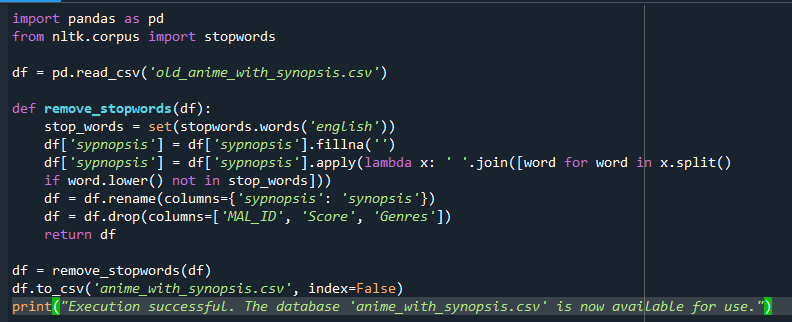
\includegraphics[scale=1]{fig1.png}
\end{flushleft}
\newpage
\section{Codificação}
\begin{flushleft}
Primeiro, importamos as bibliotecas necessárias e definimos as variáveis necessárias, incluindo o caminho do arquivo CSV e o tamanho do chunk. Em seguida, lemos o arquivo CSV e o transformamos em um DataFrame. A seguir, preenchemos as colunas vazias com uma string vazia e criamos uma matriz de token de contagem usando a função CountVectorizer. Em seguida, criamos a matriz de similaridade entre as sinopses dos animes com a função cosine similarity.
\end{flushleft}
\begin{flushleft}
Solicitamos ao usuário o título do anime que deseja buscar. O programa verifica se o título está na lista de animes e, se estiver, seleciona a sinopse do anime para calcular a similaridade com outros animes. Caso contrário, o programa sugere uma pesquisa alternativa, fornecendo títulos semelhantes com base na sinopse. Se não houver títulos semelhantes, o programa solicita uma nova pesquisa.
\end{flushleft}
\begin{flushleft}
Após a busca, o programa exibe a vetorização das palavras da sinopse do anime de entrada e os 10 animes mais similares, juntamente com o valor do ângulo de similaridade. A similaridade é calculada usando o cosseno do ângulo entre as duas sinopses.
\end{flushleft}
\begin{flushleft}
A similaridade de cosseno é um algoritmo que mede a similaridade entre vetores de alta dimensionalidade. Neste caso, cada palavra na sinopse do anime é tratada como uma dimensão e a similaridade é calculada em um espaço vetorial de alta dimensão. O algoritmo considera a frequência de cada palavra em cada sinopse e, em seguida, calcula o ângulo entre as duas sinopses para determinar a similaridade.
\end{flushleft}
\begin{flushleft}
\newpage
\section{Exemplo}
Utilizamos a palavra "Fate" em uma busca e o programa fez a correção para "Fate/stay night", resultando na localização exata de 85 dimensões, ou seja, 85 palavras presentes no anime "Fate/stay night" e em outras sinopses armazenadas no banco de dados, além disso, o programa nos apresentou os 10 animes mais semelhantes a "Fate/stay night", como ilustrado nas imagens abaixo.
\end{flushleft}
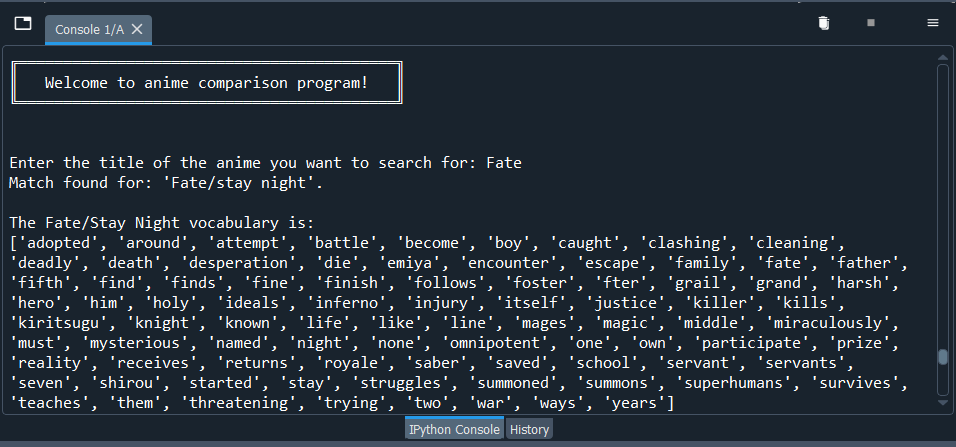
\includegraphics[scale=0.9]{R1.png}
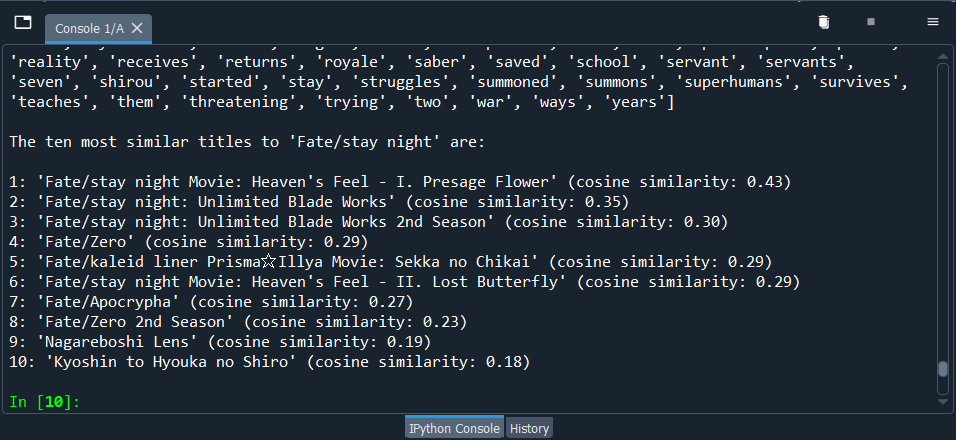
\includegraphics[scale=0.9]{R2.png}
\end{document}